
%%
%% Tokalator: A Context Engineering Toolkit for AI Coding Assistants
%%

\documentclass[preprint,12pt,a4paper]{elsarticle}

\usepackage{amssymb}
\usepackage{hyperref}
\usepackage{booktabs}
\usepackage{amsmath}
\usepackage{nicefrac}
\usepackage{listings}
\usepackage{xcolor}
\usepackage{graphicx}
\usepackage{float}
\usepackage{tikz}

% --- Order and Method: TikZ Libraries ---
\usetikzlibrary{arrows.meta, positioning, shapes.geometric}

% --- The Missing Colors: Defined at last! ---
\definecolor{extblue}{RGB}{0, 102, 204}
\definecolor{webgreen}{RGB}{0, 128, 0}
\definecolor{catpurple}{RGB}{128, 0, 128}
\definecolor{sharedgray}{RGB}{169, 169, 169}
\definecolor{codebg}{HTML}{F8F8F8}
\definecolor{codeframe}{HTML}{DDDDDD}

\setlength{\parindent}{0pt}

% --- Polished Listing Configuration ---
\lstset{
  backgroundcolor=\color{codebg},
  frame=single,
  rulecolor=\color{codeframe},
  basicstyle=\ttfamily\small,
  breaklines=true,
  tabsize=2,
  showstringspaces=false,
  numbers=left,
  numberstyle=\tiny\color{gray},
  keywordstyle=\color{extblue},      % Uses your defined color
  commentstyle=\color{webgreen},    % Uses your defined color
  stringstyle=\color{catpurple},    % Uses your defined color
  xleftmargin=1.5em,
  framexleftmargin=1.5em,
}

\journal{SoftwareX}

\begin{document}
\renewcommand{\labelenumii}{\arabic{enumi}.\arabic{enumii}}

\begin{frontmatter}

\title{Tokalator: A Context Engineering Toolkit for AI Coding Assistants}

\author[1]{Vahid Farajijobehdar\corref{cor1}}
\cortext[cor1]{Corresponding author}
\ead{vfaraji89@gmail.com}
\author[1]{Iknur Koseo\u{g}lu Sar\i{}}
\address[1]{Kariyer.net, Istanbul, Turkey}

\author[2]{Engin Zeydan}
\address[2]{Centre Tecnol\`ogic de Telecomunicacions de Catalunya (CTTC), Barcelona, Spain}

\begin{abstract}
Large language model coding assistants operate within finite context windows of 128\,K to 1\,M tokens (as of early 2026), and although providers continue to expand these limits, the core challenge persists: when developers open many files, assistant attention degrades and API costs grow super-linearly, creating an urgent need for context-aware optimization tools.

To address this gap, we present Tokalator, an open-source context engineering toolkit comprising (1)~a VS~Code extension (targeting GitHub Copilot) that monitors token budgets in real time, scores tab relevance, and exposes an interactive chat participant; (2)~a web platform with seven interactive calculators grounded in a Cobb--Douglas quality-of-output production function; and (3)~a reusable catalog of context engineering prompts, agents, and instructions.
The toolkit covers 15 models across three providers (Anthropic, OpenAI, Google), provides closed-form solutions for optimal token allocation and caching break-even analysis, and supports three multi-turn conversation cost strategies with formal cost models.

\end{abstract}

\begin{keyword}
context engineering \sep token economics \sep LLM cost optimization \sep context window 
\end{keyword}

\end{frontmatter}

\section*{Motivation}

Modern AI coding assistants such as GitHub Copilot, Claude Code, Cursor and other integrated development environment (IDE) are a gateway as software applications that help programmers develop software code efficiently. 


The ``State of AI'' empirical study~\cite{aubakirova2025state}, based on over 100 trillion tokens of real-world interactions on the OpenRouter platform, reveals a massive shift in how large LLMs are consumed. This consumption is increasingly dominated by agentic workflows, technical tasks, and reasoning-heavy models. Average prompt tokens per request grew nearly 4x (from ~1.5K to over 6K) between early 2024 and late 2025. Completion tokens nearly tripled (from ~150 to 400), leading to a total average sequence length of over 5,400 tokens by late 2025

The IDE now are powered by providers of LLMs with context size ranging from 128\,K to 1\,M tokens (Up to 2026, Feb). Despite this fact and huge context size, developers have no visibility into how their context budget is spent. Every open tab(s), system prompt(s), instruction files, and conversations turn consumes part of this budget. For example, Anthropic's Claude Opus~4.6 pricing of \$5.00 per million input tokens and \$25.00 per million output tokens, a single 200\,K-token prompt costs \$1.00 in input alone.


Existing tools address fragments of this problem: \texttt{tiktoken}~\cite{sennrich2016bpe} and Anthropic's tokenizer provide token counts, but neither integrates real-time budget visualization, multi-provider cost comparison, or economic optimization.
Bergemann et al.~\cite{bergemann2025economics} introduced a Cobb--Douglas production function framework for LLM economics, but provided no developer-facing implementation. The consequences are threefold:
\begin{enumerate}
  \item \textbf{Attention dilution}: irrelevant files compete with relevant ones, degrading output quality~\cite{bergemann2025economics}.
  \item \textbf{Cost escalation}: multi-turn conversations with full history grow at $O(t^2)$ cumulative cost, because at turn~$t$ the model receives $S + t(u + a)$ input tokens (system prompt~$S$, average user tokens~$u$, average assistant tokens~$a$), so cumulative input cost is proportional to $\sum_{t=1}^{T}[S + t(u+a)] = ST + \tfrac{T(T+1)}{2}(u+a) \in O(T^2)$.
  \item \textbf{Context rot}: after 20+ turns, stale context introduces inconsistencies.
\end{enumerate}


To address this gap, we present Tokalator as abbreviation of token calculator to bridges the gap of visualize the hidden token, context and how to manage them effectively. This extension toolkit aims to combine real-time context budget monitoring (for now VS~Code extension), interactive economic optimization tools (web platform), and reusable context engineering artifacts (prompt/agent catalog) into a unified, free, open-source package.
The extension activates on startup of IDE and passively monitors the developer's context budget, requiring no configuration to provide immediate value.

%% Meta DATA 
\section*{Metadata}

\label{sec:metadata}

\begin{table}[!h]
\begin{tabular}{|l|p{6.5cm}|p{6.5cm}|}
\hline
\textbf{Nr.} & \textbf{Code metadata description} & \textbf{Metadata} \\
\hline
C1 & Current code version & v0.2.6 \\
\hline
C2 & Permanent link to code/repository used for this code version & \url{https://github.com/vfaraji89/tokalator} \\
\hline
C3 & Permanent link to Reproducible Capsule & N/A \\
\hline
C4 & Legal Code License & MIT License \\
\hline
C5 & Code versioning system used & git \\
\hline
C6 & Software code languages, tools, and services used & TypeScript, JavaScript, Next.js~16, React~19, Tailwind~CSS~4, Recharts, Prisma~7, VS~Code Extension API, esbuild \\
\hline
C7 & Compilation requirements, operating environments \& dependencies & Node.js~$\geq$18, VS~Code~$\geq$1.99; Web: Next.js~16, React~19; Extension: \texttt{@anthropic-ai/tokenizer}, \texttt{js-tiktoken} \\
\hline
C8 & If available Link to developer documentation/manual & \url{https://tokalator.wiki/extension} \\
\hline
\end{tabular}
\caption{Code metadata (mandatory).}
\label{codeMetadata}
\end{table}

\begin{table}[!h]
\begin{tabular}{|l|p{6.5cm}|p{6.5cm}|}
\hline
\textbf{Nr.} & \textbf{(Executable) software metadata description} & \textbf{Please fill in this column} \\
\hline
S1 & Current software version & 0.2.6 \\
\hline
S2 & Permanent link to executables of this version & \url{https://marketplace.visualstudio.com/items?itemName=vfaraji89.tokalator} \\
\hline
S3 & Permanent link to Reproducible Capsule & N/A \\
\hline
S4 & Legal Software License & MIT License \\
\hline
S5 & Computing platforms/Operating Systems & Windows, macOS, Linux (any OS supporting VS~Code~$\geq$1.99); Web platform: any modern browser \\
\hline
S6 & Installation requirements \& dependencies & VS~Code~$\geq$1.99 for the extension; Node.js~$\geq$18 for the web platform \\
\hline
S7 & If available, link to user manual & \url{https://tokalator.wiki/extension} \\
\hline
S8 & Support email for questions & vahid.faraji89@gmail.com \\
\hline
\end{tabular}
\caption{Software metadata (optional).}
\label{executabelMetadata}
\end{table}


%% ─── RELATED WORK ─────────────────────────────────────────
\section{Related work}
\label{sec:related}

Several lines of work relate to Tokalator's scope.

\textbf{Tokenization libraries.}
OpenAI's \texttt{tiktoken} and Anthropic's \texttt{claude-tokenizer} provide programmatic token counting for their respective BPE vocabularies~\cite{sennrich2016bpe}. These are low-level libraries; neither offers real-time IDE integration, multi-provider comparison, or cost estimation.

\textbf{LLM pricing and inference economics.}
Bergemann, Bonatti, and Smolin~\cite{bergemann2025economics} formalized LLM output quality as a Cobb--Douglas production function of input, output, and cached tokens, but provided no implementation.
Erdil~\cite{erdil2025pareto} analyzed Pareto frontiers of inference cost versus capability, while Cottier et al.~\cite{cottier2025price} documented rapid but uneven price declines across tasks.
Yotta Labs~\cite{yotta2026econ} examined inference economics beyond per-token pricing.
These works provide economic theory but no developer-facing tools.

\textbf{Context window research.}
The ``State of AI'' study by Aubakirova et al.~\cite{aubakirova2025state} documented a $\sim$4$\times$ growth in average prompt length on OpenRouter (from 1.5\,K to 6\,K tokens) between 2024--2025, driven by agentic workflows.
Emberson et al.~\cite{emberson2025length} showed that LLM responses to benchmark questions are growing longer over time, further increasing context pressure.
Burnham and Adamczewski~\cite{burnham2025context} introduced the term ``context engineering'' to describe the systematic design of what enters the context window.

\textbf{Developer tools.}
To our knowledge, no existing open-source tool integrates real-time context budget monitoring inside an IDE with multi-provider cost comparison and economic optimization.
Commercial tools such as Cursor and Windsurf provide some internal context management, but these are opaque and not user-configurable.

%% SOFTWARE DESCRIPTION 
\section{Software description}
\label{sec:description}

\subsection{Software architecture}
\label{sec:architecture}

Tokalator comprises three independently deployable components (Figure~\ref{fig:arch}):

\begin{enumerate}
  \item \textbf{VS~Code Extension} (TypeScript, $\sim$2,700 LOC): Real-time context budget monitoring with 13 model profiles (4~Anthropic, 6~OpenAI, 3~Google), tab relevance scoring, sidebar dashboard, and an interactive chat participant (\texttt{@tokalator}).
  \item \textbf{Web Platform} (Next.js~16 + React~19): Seven interactive calculators covering 15 models across three providers, a 10-lesson context engineering course, a wiki with automated article aggregation, and a dictionary of 41 terms.
  \item \textbf{Context Engineering Catalog} (Markdown/YAML): A growing collection of reusable agents, prompts, instructions, and collections auto-discovered from \texttt{copilot-contribution/} and \texttt{user-content/} directories using file-extension conventions (\texttt{.agent.md}, \texttt{.prompt.md}, \texttt{.instructions.md}, \texttt{.collection.yml}).
\end{enumerate}

\begin{figure}[H]
\centering
\small
\begin{verbatim}
 +-------------------+--------------------+----------------+
 |  VS Code Extension|   Web Platform     |  Catalog       |
 |  (TypeScript)     |   (Next.js 16)     |  (Markdown)    |
 +-------------------+--------------------+----------------+
 | Context Monitor   | Cost Calculator    | Agents (.agent)|
 | Tokenizer Service | Context Optimizer  | Prompts(.prompt|
 | Relevance Scorer  | Model Comparison   | Instructions   |
 | Chat Participant  | Caching ROI        | Collections    |
 | Dashboard Webview | Conversation Est.  |                |
 | Status Bar        | Economic Analysis  |                |
 |                   | Usage Tracker      |                |
 +-------------------+--------------------+----------------+
 |        Shared: lib/pricing, lib/context,                |
 |        lib/caching, lib/conversation                    |
 |        lib/providers (15 models, 3 providers)           |
 +------------------+--------------------------------------+
\end{verbatim}
\caption{Tokalator system architecture. Three independent components share a library layer providing pricing, context analysis, caching, and conversation estimation. The web platform covers 15 models and the extension supports 13 model profiles across Anthropic, OpenAI, and Google.}
\label{fig:arch}
\end{figure}

The web platform's library layer (\texttt{lib/pricing}, \texttt{lib/caching}, \texttt{lib/conversation}, \texttt{lib/context}) provides the computational backend for all seven calculators.
The VS~Code extension maintains its own embedded model profiles and tokenizer logic (\texttt{modelProfiles.ts}, \texttt{tokenizerService.ts}) because it runs inside the extension host process and cannot import Next.js modules; both implementations track the same provider pricing but are maintained independently.

The extension's internal architecture follows a four-layer design:
\begin{itemize}
  \item \textbf{Core Engine} (\texttt{contextMonitor.ts}): subscribes to VS~Code editor events (active editor changes, tab open/close, document edits, diagnostic updates), builds \texttt{ContextSnapshot} records, and manages pinned files and model selection via \texttt{workspaceState}. All event handlers are debounced (300\,ms) to avoid performance overhead from rapid event firing.
  \item \textbf{Tokenizer Service} (\texttt{tokenizerService.ts}): provider-specific BPE tokenizers---\texttt{claude-tokenizer} for Anthropic, \texttt{js-tiktoken} (\texttt{o200k\_base}) for OpenAI, heuristic ($\sim$4~chars/token) for Google. Tokenizers are lazy-loaded on first use and results are cached per-document keyed by URI and document version, so re-tokenization occurs only when the file changes.
  \item \textbf{Relevance Scorer} (\texttt{tabRelevanceScorer.ts}): scores each open tab $R \in [0, 1]$ based on five weighted signals: language match ($+0.25$), import analysis ($+0.30$), path similarity ($+0.20$), edit recency ($+0.15$), and diagnostic count ($+0.10$). Pinned and active tabs are overridden to $R = 1.0$.
  \item \textbf{Chat Participant} (\texttt{contextChatParticipant.ts}): registers \texttt{@tokalator} with ten slash commands.
\end{itemize}

The central data structure is \texttt{ContextSnapshot}, emitted on every state change, containing: a timestamp, the active file, a list of all open tabs (each with URI, estimated tokens, relevance score, and diagnostics), the set of pinned files, total estimated tokens, window capacity, usage percentage, budget level (\texttt{low}/\texttt{medium}/\texttt{high}), context health status with reasons, model identifier, workspace-level file statistics, the tokenizer type in use, per-turn history, and a \texttt{BudgetBreakdown} struct that itemizes files, system prompt, instructions, conversation, and output reservation.


%% ── UML Sequence Diagram ──────────────────────────────────
\begin{figure}[H]
\centering
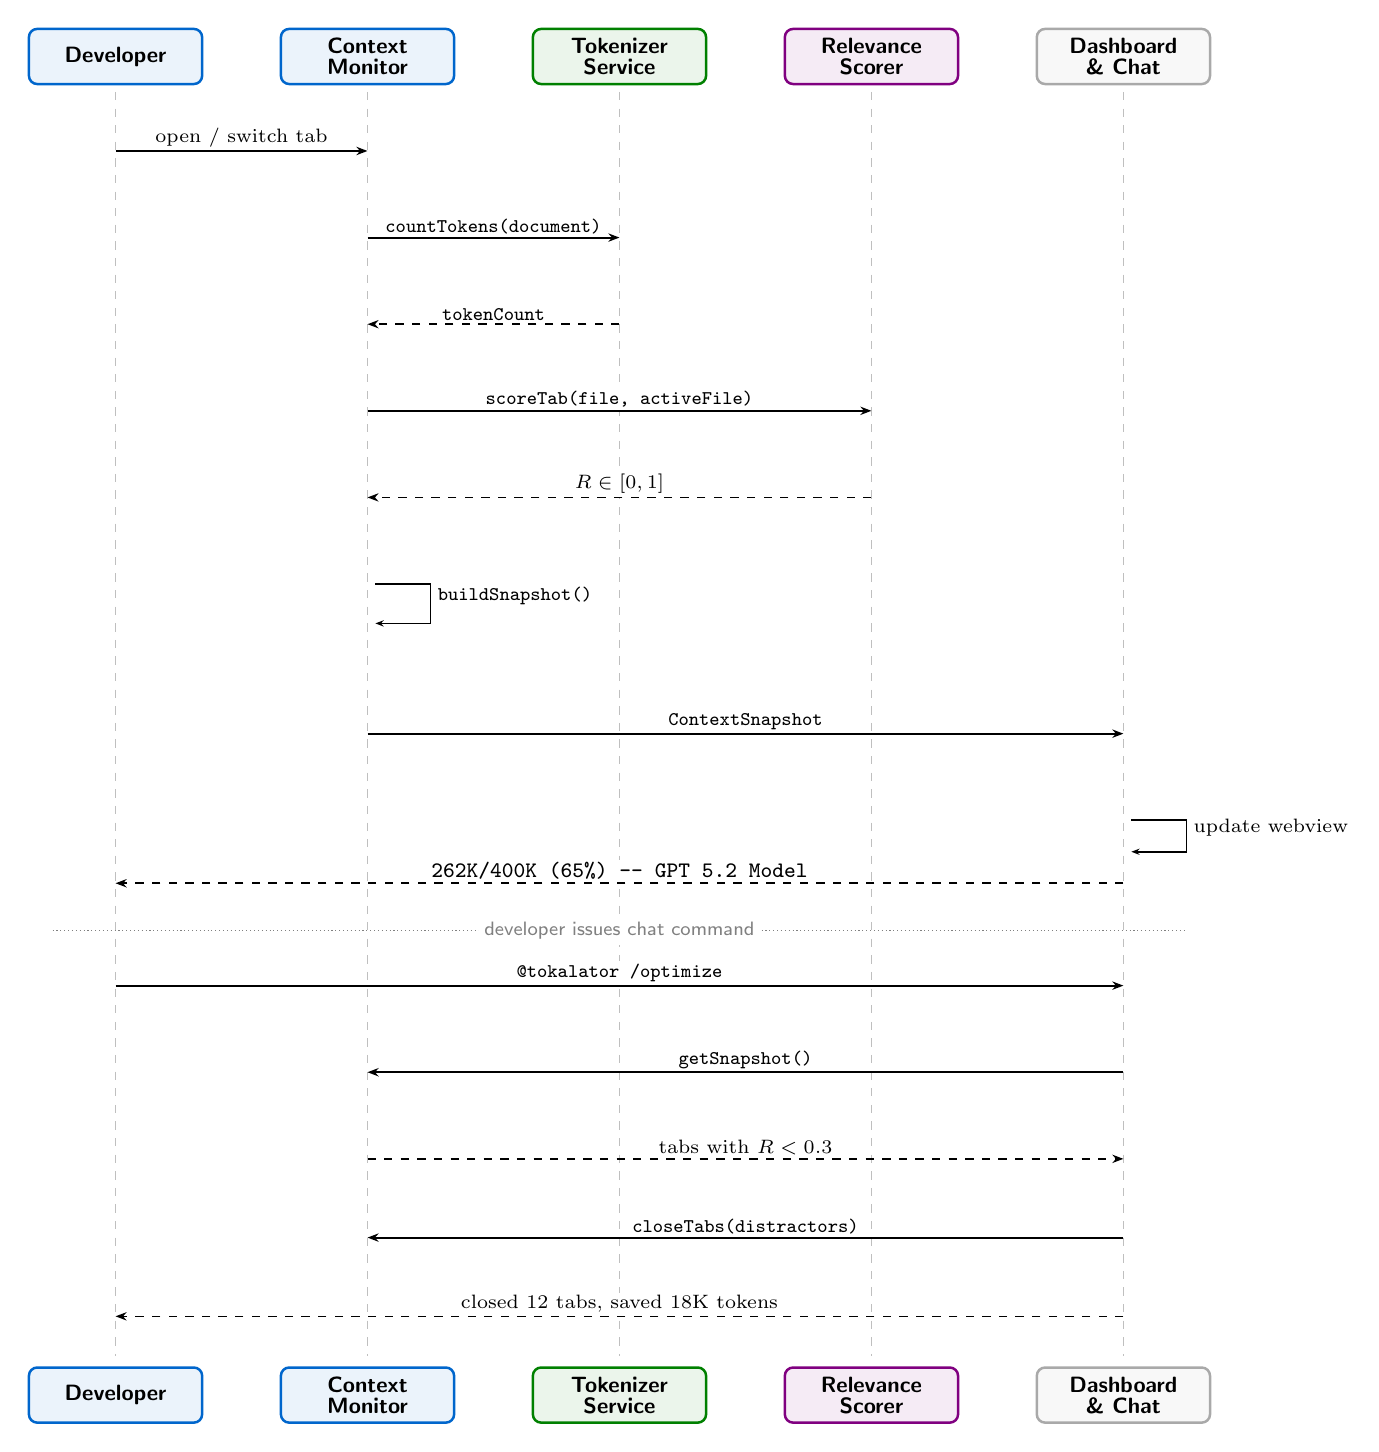
\begin{tikzpicture}[
  >=Stealth,
  actor/.style={
    rectangle, rounded corners=3pt, draw=#1, fill=#1!8,
    line width=0.9pt, minimum height=0.7cm, minimum width=2.2cm,
    font=\footnotesize\sffamily\bfseries, align=center
  },
  msg/.style={font=\scriptsize, fill=white, inner sep=1pt},
  lifeline/.style={dashed, draw=gray!50, line width=0.5pt},
  call/.style={-{Stealth[length=4pt]}, line width=0.7pt},
  ret/.style={-{Stealth[length=4pt]}, dashed, line width=0.6pt},
  selfarrow/.style={-{Stealth[length=3pt]}, line width=0.6pt},
]

\def\colA{0}
\def\colB{3.2}
\def\colC{6.4}
\def\colD{9.6}
\def\colE{12.8}

\node[actor=extblue]   (devT)  at (\colA, 0) {Developer};
\node[actor=extblue]   (monT)  at (\colB, 0) {Context\\[-2pt]Monitor};
\node[actor=webgreen]  (tokT)  at (\colC, 0) {Tokenizer\\[-2pt]Service};
\node[actor=catpurple] (relT)  at (\colD, 0) {Relevance\\[-2pt]Scorer};
\node[actor=sharedgray](uiT)   at (\colE, 0) {Dashboard\\[-2pt]\& Chat};

\def\bottom{-16.5}
\draw[lifeline] (\colA, -0.45) -- (\colA, \bottom);
\draw[lifeline] (\colB, -0.45) -- (\colB, \bottom);
\draw[lifeline] (\colC, -0.45) -- (\colC, \bottom);
\draw[lifeline] (\colD, -0.45) -- (\colD, \bottom);
\draw[lifeline] (\colE, -0.45) -- (\colE, \bottom);

\def\rA{-1.2}
\def\rB{-2.3}
\def\rC{-3.4}
\def\rD{-4.5}
\def\rE{-5.6}
\def\rF{-6.7}
\def\rG{-7.8}
\def\rH{-8.6}
\def\rI{-9.7}
\def\rJ{-10.5}
\def\rK{-11.8}
\def\rL{-12.9}
\def\rM{-14.0}
\def\rN{-15.0}
\def\rO{-16.0}

% 1. Developer opens/switches a tab
\draw[call] (\colA, \rA) -- node[msg, above] {open / switch tab} (\colB, \rA);

% 2. Monitor requests token count
\draw[call] (\colB, \rB) -- node[msg, above] {\texttt{countTokens(document)}} (\colC, \rB);

% 3. Tokenizer returns count
\draw[ret] (\colC, \rC) -- node[msg, above] {\texttt{tokenCount}} (\colB, \rC);

% 4. Monitor requests relevance score
\draw[call] (\colB, \rD) -- node[msg, above] {\texttt{scoreTab(file, activeFile)}} (\colD, \rD);

% 5. Scorer returns relevance
\draw[ret] (\colD, \rE) -- node[msg, above] {$R \in [0, 1]$} (\colB, \rE);

% 6. Monitor builds snapshot (self-call)
\draw[selfarrow] (\colB+0.1, \rF) -- ++(0.7, 0) -- ++(0, -0.5) -- ++(-0.7, 0);
\node[msg, right] at (\colB+0.85, \rF-0.15) {\texttt{buildSnapshot()}};

% 7. Monitor sends snapshot to Dashboard
\draw[call] (\colB, \rH) -- node[msg, above] {\texttt{ContextSnapshot}} (\colE, \rH);

% 8. Dashboard updates UI
\draw[selfarrow] (\colE+0.1, \rI) -- ++(0.7, 0) -- ++(0, -0.4) -- ++(-0.7, 0);
\node[msg, right] at (\colE+0.85, \rI-0.1) {update webview};

% 9. Dashboard updates status bar
\draw[ret] (\colE, \rJ) -- node[msg, above] {\footnotesize\texttt{262K/400K (65\%) -- GPT 5.2 Model}} (\colA, \rJ);

% Separator
\draw[densely dotted, gray] (-0.8, -11.1) -- (13.6, -11.1);
\node[font=\scriptsize\sffamily, gray, fill=white, inner sep=2pt] at (6.4, -11.1) {developer issues chat command};

% 10. Developer sends @tokalator /optimize
\draw[call] (\colA, \rK) -- node[msg, above] {\texttt{@tokalator /optimize}} (\colE, \rK);

% 11. Chat requests current snapshot
\draw[call] (\colE, \rL) -- node[msg, above] {\texttt{getSnapshot()}} (\colB, \rL);

% 12. Monitor returns snapshot with low-R tabs
\draw[ret] (\colB, \rM) -- node[msg, above] {tabs with $R < 0.3$} (\colE, \rM);

% 13. Chat closes low-relevance tabs
\draw[call] (\colE, \rN) -- node[msg, above] {\texttt{closeTabs(distractors)}} (\colB, \rN);

% 14. Result to developer
\draw[ret] (\colE, \rO) -- node[msg, above] {closed 12 tabs, saved 18K tokens} (\colA, \rO);

% Actor boxes (bottom)
\node[actor=extblue]   at (\colA, \bottom-0.5) {Developer};
\node[actor=extblue]   at (\colB, \bottom-0.5) {Context\\[-2pt]Monitor};
\node[actor=webgreen]  at (\colC, \bottom-0.5) {Tokenizer\\[-2pt]Service};
\node[actor=catpurple] at (\colD, \bottom-0.5) {Relevance\\[-2pt]Scorer};
\node[actor=sharedgray]at (\colE, \bottom-0.5) {Dashboard\\[-2pt]\& Chat};

\end{tikzpicture}
\caption{Sequence diagram of the Tokalator VS~Code extension workflow. \textbf{Top half}: when the developer opens or switches a tab, the Context Monitor requests token counts and relevance scores, builds a \texttt{ContextSnapshot}, and pushes it to the Dashboard and status bar. \textbf{Bottom half}: when the developer issues \texttt{@tokalator /optimize}, the Chat Participant retrieves the snapshot, identifies tabs with relevance $R < 0.3$, and closes them.}
\label{fig:seq}
\end{figure}

\subsection{Software functionalities}
\label{sec:functionalities}

\subsubsection{VS~Code Extension}

The extension provides five core functionalities:

\textbf{1. Real-time token budget monitoring.}
The status bar displays a continuously updated summary: \texttt{\$(check) 262K / 400K (6.2\%) -- Open AI 5.2 Model}.
A sidebar webview dashboard shows the full breakdown: budget level (low/medium/high), per-file token estimates, pinned file count, conversation turn count, and context health warnings.

The total estimated tokens are computed as the sum of five components:
\begin{equation}
  T_{\text{total}} = T_{\text{files}} + T_{\text{sys}} + T_{\text{instr}} + T_{\text{conv}} + T_{\text{out}}
\end{equation}
where $T_{\text{files}} = \sum_i \text{tokens}(\text{tab}_i)$ is the sum of per-file BPE token counts across all open tabs, $T_{\text{sys}} = 2{,}000$ is the estimated system prompt overhead (Copilot's hidden system prompt), $T_{\text{instr}} = 500 \times n_{\text{instr}}$ accounts for instruction files detected in the workspace, $T_{\text{conv}} = 800 \times t$ estimates accumulated conversation history at turn~$t$, and $T_{\text{out}} = 4{,}000$ reserves tokens for the model's response.
These overhead constants are informed by empirical measurement of GitHub Copilot's context construction but are necessarily approximate since the actual assistant context logic is proprietary (see Section~\ref{sec:limitations}).

\textbf{2. Tab relevance scoring.}
Each open tab receives a relevance score $R \in [0, 1]$ computed as a weighted sum of five signals:
\begin{equation}
  R = 0.25\,S_{\text{lang}} + 0.30\,S_{\text{import}} + 0.20\,S_{\text{path}} + 0.15\,S_{\text{recency}} + 0.10\,S_{\text{diag}}
\end{equation}
where $S_{\text{lang}} \in \{0, 1\}$ indicates language match with the active file, $S_{\text{import}} \in \{0, 1\}$ indicates an import relationship, $S_{\text{path}} \in [0, 1]$ measures shared directory depth (computed as the ratio of shared path prefix segments to total depth), $S_{\text{recency}} \in \{0, 0.53, 1\}$ reflects edit recency (1.0 if edited within 2 minutes, 0.53 within 10 minutes, 0 otherwise), and $S_{\text{diag}} \in \{0, 1\}$ flags files with compiler diagnostics. Pinned and active files are overridden to $R = 1.0$.

The weights were assigned based on the following design rationale: import relationships ($w=0.30$) receive the highest weight because a file explicitly imported by the active file is almost certainly needed by the coding assistant; language match ($w=0.25$) is the next strongest signal since cross-language files (e.g., \texttt{.json} configs open alongside \texttt{.tsx} code) are common distractors; path similarity ($w=0.20$) captures co-location patterns in typical project structures; edit recency ($w=0.15$) reflects the developer's current working set; and diagnostics ($w=0.10$) provide a weak signal that files with errors are being actively debugged.
The $S_{\text{recency}}$ intermediate value of~0.53 corresponds to $\nicefrac{0.08}{0.15}$, the ratio of the partial recency credit (0.08 for files edited within 10 minutes) to the full recency weight.
The default distractor threshold of $R < 0.3$ was chosen so that a file must match on at least two signals (e.g., same language + nearby path) to avoid being flagged.
These weights are configurable and could benefit from empirical calibration in future work.
Tabs scoring below the threshold are flagged as distractors.

\textbf{3. Chat participant with ten commands.}
The \texttt{@tokalator} chat participant responds to: \texttt{/count} (budget status), \texttt{/breakdown} (per-file tokens), \texttt{/optimize} (close low-relevance tabs), \texttt{/pin}/\texttt{/unpin} (pin management), \texttt{/instructions} (scan instruction files and their token cost), \texttt{/model} (switch model profile), \texttt{/compaction} (per-turn growth analysis), \texttt{/reset} and \texttt{/exit} (session management).

\textbf{4. Session persistence.}
Session summaries (peak tokens, turns, model, top edited files) are saved to \texttt{workspaceState} on exit and shown as a notification on the next activation.
Pinned files and model selection persist across VS~Code restarts.

\textbf{5. Instruction file scanner.}
The extension detects and tokenizes instruction files automatically injected into prompts: \texttt{.github/copilot-instructions.md}, \texttt{CLAUDE.md}, \texttt{AGENTS.md}, \texttt{.cursorrules}, and \texttt{.instructions.md} files, revealing their hidden token cost.

\subsubsection{Web Platform}

The web platform at \url{https://tokalator.wiki} provides seven interactive tools:

\begin{enumerate}
  \item \textbf{Cost Calculator}: Token cost calculation with Cobb--Douglas quality modeling for Anthropic, OpenAI, and Google models. Supports tiered pricing detection: when the total prompt length exceeds Anthropic's 200\,K-token threshold (available for Opus and Sonnet via the 1\,M context beta), \emph{all} input tokens in that request are billed at the extended rate (2$\times$ standard input cost), not only the tokens above the threshold. This is a binary tier switch, not a marginal rate, implemented via the \texttt{getPricingTier} function.

  \item \textbf{Context Optimizer}: Visualizes context window allocation across system prompt, user input, reserved output, and free space. Computes usage percentage and generates warnings.

  \item \textbf{Model Comparison}: Cross-provider cost and capability comparison across all 15 models.

  \item \textbf{Caching ROI Calculator}: Break-even analysis for prompt caching. Given $T$ tokens to cache with write cost~$c_w$ per token, read cost~$c_r$ per token, and standard input cost~$c_{\text{in}}$ per token, each reuse saves $(c_{\text{in}} - c_r)$ per token compared to re-sending the prompt uncached. The break-even reuse count is:
  \begin{equation}
    n^* = \left\lceil \frac{c_w}{c_{\text{in}} - c_r} \right\rceil
  \end{equation}
  For all current Anthropic models, $c_w = 1.25 \times c_{\text{in}}$ and $c_r = 0.10 \times c_{\text{in}}$, yielding $n^* = \lceil 1.25 / 0.90 \rceil = 2$ reuses. At 10 reuses the savings reach 76\%.

  \item \textbf{Conversation Estimator}: Multi-turn cost projection under three strategies, each defined by the input tokens sent at turn~$t$ (with system prompt~$S$, average user tokens~$u$, average assistant tokens~$a$):
  \begin{itemize}
    \item \textbf{Full History}: $I_t = S + \sum_{i=1}^{t}(u_i + a_i)$, yielding $O(T^2)$ cumulative cost since $\sum_{t=1}^{T} I_t = ST + \tfrac{T(T+1)}{2}(u+a)$.
    \item \textbf{Sliding Window} ($W$ turns): $I_t = S + \sum_{i=\max(1,\,t-W+1)}^{t}(u_i + a_i)$, capping per-turn cost at $S + W(u+a)$ for $t \geq W$, yielding $O(T)$ cumulative cost.
    \item \textbf{Summarize} (ratio $\rho$, keep last $k$ turns fresh): $I_t = S + \rho \cdot \sum_{i=1}^{t-k}(u_i + a_i) + \sum_{i=t-k+1}^{t}(u_i + a_i)$, growing slowly at rate $\rho(u+a)$ per turn.
  \end{itemize}
  Per-turn breakdown charts visualize the cost trajectories.

  \item \textbf{Economic Analysis}: Visualization of the Cobb--Douglas quality-of-output production function:
  \begin{equation}
    Q(X, Y, Z) = X^{\alpha} \cdot Y^{\beta} \cdot (b + Z)^{\gamma}
  \end{equation}
  where $X$ = input tokens, $Y$ = output tokens, $Z$ = cache/fine-tuning tokens, $b$ = base model quality, and $\alpha, \beta, \gamma$ are provider-specific sensitivity parameters ($\alpha + \beta + \gamma < 1$, ensuring diminishing returns to scale).

  The corresponding cost minimization problem is:
  \begin{equation}
    \min_{X,Y,Z \geq 0} \; c_x X + c_y Y + c_z Z \qquad \text{s.t.} \quad Q(X,Y,Z) \geq \bar{Q}
  \end{equation}
  where $c_x, c_y, c_z$ are the per-token costs for input, output, and cache-write respectively.
  Applying the Lagrangian and the first-order conditions (equating marginal-product-per-dollar ratios), the optimal allocation satisfies $X^*/Y^* = (\alpha\, c_y) / (\beta\, c_x)$, and the minimum cost for target quality~$\bar{Q}$ without caching is:
  \begin{equation}
    C^*(\bar{Q}) = (\alpha + \beta) \left(\frac{\bar{Q}}{b^{\gamma}}\right)^{\!1/(\alpha+\beta)} \left(\frac{c_x}{\alpha}\right)^{\!\alpha/(\alpha+\beta)} \left(\frac{c_y}{\beta}\right)^{\!\beta/(\alpha+\beta)}
  \end{equation}
  following Lemma~4 of Bergemann et al.~\cite{bergemann2025economics}. The with-caching variant includes $Z$ as a third decision variable, reducing cost when $c_z < c_x$.

  The sensitivity parameters used in the implementation ($\alpha = 0.30$, $\beta = 0.35$, $\gamma = 0.20$, $b = 1.0$ for Opus; $\alpha = 0.25$, $\beta = 0.30$, $\gamma = 0.20$, $b = 0.85$ for Sonnet; $\alpha = 0.20$, $\beta = 0.25$, $\gamma = 0.15$, $b = 0.70$ for Haiku) are hypothetical values chosen to reflect the qualitative ranking of models (higher $b$ and $\alpha + \beta$ for more capable models) and to ensure $\alpha + \beta + \gamma < 1$. They are not calibrated from empirical data, as no public benchmark currently measures output quality as a function of token allocation. Users can adjust these parameters in the Economic Analysis tool to explore sensitivity.

  The tool renders quality isoquant curves and cost minimization surfaces with and without caching.

  \item \textbf{Usage Tracker}: Historical API usage analysis with cost breakdowns by model, project, and time period, plus linear regression and exponential smoothing projections.
\end{enumerate}

The platform also includes a 10-lesson context engineering course (\texttt{/learn}), a wiki with an automated monthly fetch pipeline that aggregates articles from arXiv, OpenAI Cookbook, and provider documentation, and a dictionary of 41 context engineering terms organized across eight categories.

\subsubsection{Context Engineering Catalog}

The catalog auto-discovers reusable artifacts from the repository using file extension conventions: \texttt{.agent.md} (agents), \texttt{.prompt.md} (prompts), \texttt{.instructions.md} (workspace guidelines), \texttt{.collection.yml} (bundles), and \texttt{CLAUDE.md} (Claude Code instructions).
A \texttt{user-content/} directory accepts community contributions, which are automatically indexed with YAML frontmatter parsing.


%% ─── 3. ILLUSTRATIVE EXAMPLES ─────────────────────────────
\section{Illustrative examples}
\label{sec:examples}

\textbf{Example 1: Identifying context budget waste in a VS~Code session.}
A developer working on a React project has 23 tabs open.
After installing Tokalator, the status bar shows: \texttt{\$(warning) 85.2K / 200K (42.6\%) -- Sonnet 4.5}.
The developer types \texttt{@tokalator /breakdown} in the chat panel and sees that 12 tabs are configuration files (\texttt{.json}, \texttt{.yml}) contributing 18\,K tokens but scoring below the 0.3 relevance threshold.
Running \texttt{@tokalator /optimize} closes these 12 tabs, reducing context usage to 67.2K tokens (33.6\%).
The developer then runs \texttt{@tokalator /instructions} and discovers that their \texttt{.github/copilot-instructions.md} file alone costs 4,200 tokens---injected silently into every prompt.

\textbf{Example 2: Choosing a caching strategy via the web platform.}
A team building a customer support chatbot uses a 50\,K-token system prompt (product documentation + few-shot examples).
On the Caching ROI Calculator, they enter 50\,000 cache tokens with Claude Sonnet~4.5 and 100 daily reuses.
The calculations proceed as follows (Sonnet~4.5 pricing: $c_{\text{in}} = \$3.00$/MTok, $c_w = \$3.75$/MTok, $c_r = \$0.30$/MTok):
\begin{itemize}
  \item Write cost: $50{,}000 / 10^6 \times 3.75 = \$0.19$
  \item Uncached daily cost: $101 \times 50{,}000 / 10^6 \times 3.00 = \$15.15$ (initial + 100 reuses)
  \item Cached daily cost: $\$0.19 + 100 \times 50{,}000 / 10^6 \times 0.30 = \$1.69$
  \item Net savings: $\$15.15 - \$1.69 = \$13.46$/day (88.9\%)
  \item Break-even: $\lceil 3.75 / (3.00 - 0.30) \rceil = \lceil 1.39 \rceil = 2$ reuses
\end{itemize}
The per-reuse comparison chart makes the decision obvious.

\textbf{Example 3: Planning conversation length within budget.}
A developer with a \$5 daily API budget uses the Conversation Estimator.
They configure: Claude Sonnet~4.5, 2\,000-token system prompt, 500 avg user tokens, 1\,500 avg assistant tokens per turn.
The tool shows that with Full History strategy, they can afford 28 turns before exhausting the budget, but Sliding Window (W=5) allows 83 turns and Summarize ($\rho=0.2$) allows 71 turns.
The per-turn cost chart visually shows the quadratic growth of Full History versus the linear growth of alternatives.


%% ─── 4. IMPACT ────────────────────────────────────────────
\section{Impact}
\label{sec:impact}

Tokalator addresses a gap in the AI-assisted development workflow that affects every developer using LLM coding assistants.
Its impact spans three dimensions:

\textbf{Visibility into a previously opaque resource.}
Before Tokalator, developers had no way to see how their context window was being consumed.
The extension makes token budgets as visible as memory or CPU usage in traditional development, enabling informed decisions about which files to keep open and when to start a new conversation.

\textbf{Actionable cost optimization.}
The web platform's calculators translate economic theory (Cobb--Douglas production functions, prompt caching break-even analysis) into interactive tools that require no mathematical background.
A developer can determine in seconds whether caching is worthwhile for their use case, or how many conversation turns their budget supports under different strategies.

\textbf{Educational contribution.}
The 10-lesson context engineering course, wiki, and dictionary lower the barrier to understanding token economics.
The context engineering catalog provides ready-to-use artifacts that encode best practices for structuring AI-assisted workflows.

\textbf{Ecosystem contribution.}
The catalog provides a structured framework for contributing and discovering context engineering artifacts for the GitHub Copilot ecosystem, with built-in agents, prompts, and instructions available for community reuse and extension.
The extension supports 15 models across three major providers, avoiding vendor lock-in.

The VS~Code extension is publicly available on the Marketplace and the web platform receives traffic from developers seeking context optimization guidance.
As context windows grow toward 1\,M+ tokens and AI-assisted coding becomes standard practice, the need for context budget tooling will only increase.


%% ─── 5. LIMITATIONS ───────────────────────────────────────
\section{Limitations}
\label{sec:limitations}

Several limitations should be noted.

\textbf{Approximate tokenization for Google models.}
The extension uses a heuristic of $\sim$4 characters per token for Gemini models, as Google does not publish a client-side BPE tokenizer for JavaScript. While Anthropic and OpenAI models use real BPE tokenizers (\texttt{claude-tokenizer} and \texttt{o200k\_base} respectively), the Gemini heuristic is based on the commonly observed ratio for English-heavy code corpora (where BPE tokens average 3.5--4.5 characters). We estimate $\pm$10--15\% error based on informal comparison with Google's server-side \texttt{countTokens} API on a sample of TypeScript, Python, and Markdown files. Languages with non-Latin scripts or heavily minified code would see larger deviations. This limitation is documented in the extension's dashboard via the tokenizer label display.

\textbf{Extension performance overhead.}
The extension subscribes to six VS~Code event streams (active editor, tab changes, document edits, document open/close, diagnostics, and configuration changes). To prevent UI blocking, all event handlers feed into a 300\,ms debounce timer, so at most one \texttt{refresh()} call occurs per 300\,ms burst. Token counts are cached per-document keyed by URI and version number; re-tokenization occurs only when the document content changes. The BPE tokenizers are lazy-loaded (Claude ranks: 696\,KB JSON, o200k\_base: loaded via \texttt{js-tiktoken}), adding a one-time latency of $\sim$100--200\,ms on first use. A periodic background refresh (default 2\,s, configurable) updates recency-based scores. In informal testing with 30+ open tabs, the extension contributes $<$5\,ms per snapshot build after initial tokenizer warm-up, which is imperceptible to the user.

\textbf{Syntactic rather than semantic relevance.}
The tab relevance scorer (Equation~1) uses syntactic signals---import graphs, path similarity, language match, edit recency, and diagnostics---rather than semantic code understanding. A file that is conceptually critical to the task (e.g., a specification document referenced by name in comments) will score low if it has no import relationship to the active file. Incorporating embedding-based similarity would improve accuracy but introduce latency and model dependency.

\textbf{Estimated vs.\ actual context consumption.}
The extension estimates how many tokens an AI coding assistant would include from open tabs, but the actual context construction logic of each assistant (GitHub Copilot, Cursor, Claude Code) is proprietary. The real context may include additional metadata (e.g., git diffs, terminal output) or exclude files the extension counts as open. The estimates should therefore be understood as upper-bound approximations.

\textbf{No empirical user study.}
The current version has not been validated through a controlled user study measuring the effect of context budget visibility on code quality, task completion time, or developer productivity. While the mathematical models (caching break-even, conversation cost projection) are validated through unit tests against their closed-form solutions, the end-to-end impact on developer workflows remains an open empirical question.

\textbf{Pricing volatility.}
LLM pricing changes frequently---Cottier et al.~\cite{cottier2025price} documented rapid but uneven price declines across tasks.
The toolkit's pricing data is hardcoded in \texttt{lib/providers.ts} and requires manual updates. The modular design and CI pipeline make updates straightforward, but users should verify current pricing against provider documentation.

\textbf{Single-IDE scope.}
The extension currently targets only VS~Code and GitHub Copilot. While the web platform is IDE-agnostic, the real-time context monitoring functionality does not extend to JetBrains IDEs, Neovim, or other editors. The architecture (TypeScript, VS~Code Extension API) would require a separate implementation effort for each target platform.

%% ─── 6. CONCLUSIONS ───────────────────────────────────────
\section{Conclusions}
\label{sec:conclusions}

Tokalator is the first open-source toolkit to combine real-time context budget monitoring, interactive economic optimization, and reusable context engineering artifacts for AI coding assistants.
It covers 15 models across three providers, implements prompt caching break-even analysis, supports three multi-turn conversation strategies, and provides a VS~Code extension that makes token budgets visible and actionable.
The toolkit includes a comprehensive unit test suite (110 tests covering pricing, caching, conversation simulation, context analysis, and model profile integrity) and a CI pipeline that runs build, lint, and test on every commit.

Future work includes team-wide context budget dashboards with CI/CD integration, a public token counting REST API, empirical validation of the relevance scoring algorithm's effect on LLM output quality through a controlled user study, and extension of the IDE integration to JetBrains and Neovim.

All components are MIT-licensed and available at \url{https://github.com/vfaraji89/tokalator}.


%% ─── ACKNOWLEDGEMENTS ─────────────────────────────────────
\section*{Acknowledgements}

The economic model is based on the Cobb--Douglas framework introduced by Bergemann, Bonatti, and Smolin~\cite{bergemann2025economics}.
The tokenization layer uses Anthropic's \texttt{claude-tokenizer} and OpenAI's \texttt{tiktoken}~\cite{sennrich2016bpe}.

%% ─── REFERENCES ───────────────────────────────────────────
\begin{thebibliography}{00}

\bibitem{bergemann2025economics}
D.~Bergemann, A.~Bonatti, A.~Smolin,
The Economics of Large Language Models,
Working Paper, 2025. Available at SSRN.

\bibitem{anthropic2026pricing}
Anthropic,
Claude API Pricing,
\url{https://docs.anthropic.com/en/docs/about-claude/pricing}, February 2026.

\bibitem{anthropic2025caching}
Anthropic,
Prompt Caching,
\url{https://docs.anthropic.com/en/docs/build-with-claude/prompt-caching}, 2025.

\bibitem{openai2026pricing}
OpenAI,
API Pricing,
\url{https://openai.com/api/pricing/}, February 2026.

\bibitem{google2026pricing}
Google,
Gemini API Pricing,
\url{https://ai.google.dev/pricing}, February 2026.

\bibitem{sennrich2016bpe}
R.~Sennrich, B.~Haddow, A.~Birch,
Neural Machine Translation of Rare Words with Subword Units,
in: Proceedings of ACL, 2016.

\bibitem{vscode2026api}
Microsoft,
VS~Code Extension API,
\url{https://code.visualstudio.com/api}, 2026.


\bibitem{aubakirova2025state} Aubakirova, M., et al. (2025). \textit{State of AI: An Empirical 100 Trillion Token Study with OpenRouter}.

\bibitem{burnham2025context} Burnham, G. \& Adamczewski, T. (2025). \textit{Context Engineering for AI Agents: Lessons from Building Real-World Systems}. Anthropic Research Blog.

\bibitem{emberson2025length} Emberson, L., et al. (2025). \textit{LLM responses to benchmark questions are getting longer over time}. Epoch AI.
\bibitem{erdil2025pareto} Erdil, E. (2025). \textit{Pareto Frontiers of Language Model Inference Economics}. Epoch AI.
\bibitem{cottier2025price} Cottier, B., et al. (2025). \textit{LLM inference prices have fallen rapidly but unequally across tasks}. Epoch AI.
\bibitem{yotta2026econ} Yotta Labs. (2026). \textit{The Economics of LLM Inference: Beyond Cost Per Token}.
\end{thebibliography}

\end{document}
